%!TEX root = ../../../report.tex

\begin{figure}[H]
    \newcommand{\figurewidth}{0.5\textwidth}
    \newcommand{\figureheight}{3cm}
	\begin{subfigure}[b]{\figurewidth}
        \centering
        \raisebox{0.5\height}{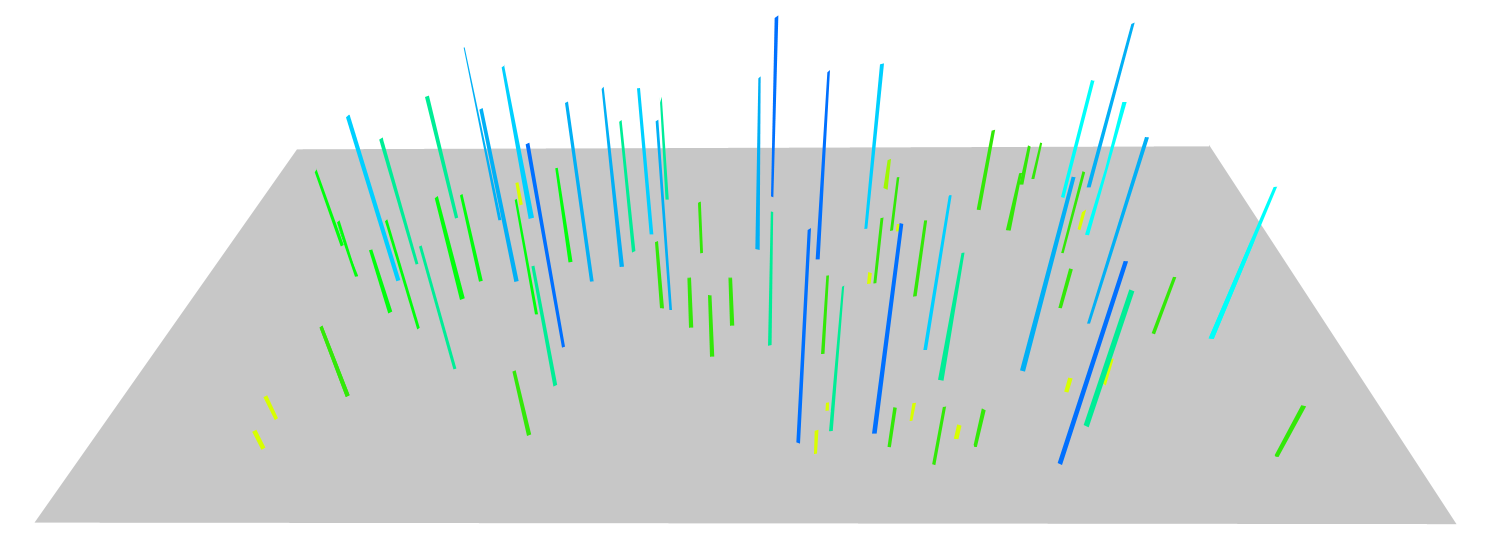
\includegraphics[width=\textwidth]{images/design/mockups/flat}}
        \caption{Visualisation using a flat surface.}
        \label{fig:visualisation_flat}
    \end{subfigure}
    \begin{subfigure}[b]{\figurewidth}
        \centering
        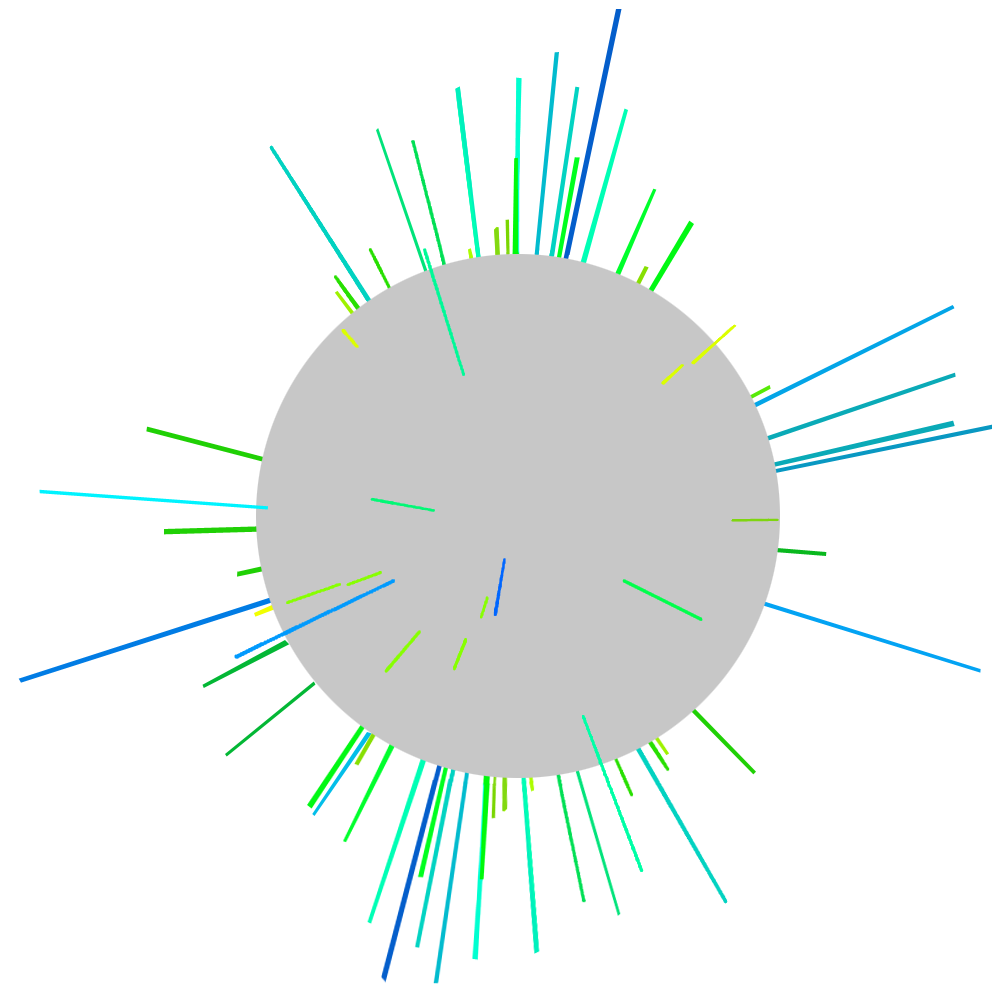
\includegraphics[width=\textwidth]{images/design/mockups/sphere}
        \caption{Visualisation using a sphere surface.}
        \label{fig:visualisation_sphere}
    \end{subfigure}
	\caption[3D environment mockups]{3D environment mockups.}
	\label{fig:environment_mockups}
\end{figure}
